\documentclass[a4paper,14pt]{extarticle}

\usepackage[utf8x]{inputenc}
\usepackage[T1,T2A]{fontenc}
\usepackage[russian]{babel}
\usepackage{hyperref}
\usepackage{indentfirst}
\usepackage{here}
\usepackage{array}
\usepackage{graphicx}
\usepackage{caption}
\usepackage{subcaption}
\usepackage{chngcntr}
\usepackage{amsmath}
\usepackage{amssymb}
\usepackage{pgfplots}
\usepackage{pgfplotstable}
\usepackage[left=2cm,right=2cm,top=2cm,bottom=2cm,bindingoffset=0cm]{geometry}
\usepackage{multicol}

\renewcommand{\le}{\ensuremath{\leqslant}}
\renewcommand{\leq}{\ensuremath{\leqslant}}
\renewcommand{\ge}{\ensuremath{\geqslant}}
\renewcommand{\geq}{\ensuremath{\geqslant}}
\renewcommand{\epsilon}{\ensuremath{\varepsilon}}
\renewcommand{\phi}{\ensuremath{\varphi}}

\counterwithin{figure}{section}
\counterwithin{equation}{section}
\counterwithin{table}{section}
\newcommand{\sign}[1][5cm]{\makebox[#1]{\hrulefill}} % Поля подписи и даты
\graphicspath{{pics/}} % Путь до папки с картинками
\captionsetup{justification=centering,margin=1cm}
\def\arraystretch{1.3}

\begin{document}	% начало документа

\begin{titlepage}
\begin{center}
	\textbf{Санкт-Петербургский Политехнический Университет \\Петра Великого}\\[0.3cm]
	\small Институт компьютерных наук и технологий \\[0.3cm]
	\small Кафедра компьютерных систем и программных технологий\\[4cm]
	
	\textbf{ОТЧЕТ}\\ \textbf{о лабораторной работе}\\[0.5cm]
	\textbf{<<Исследование частотных характеристик пассивных RC-цепей>>}\\[0.1cm]
	\textbf{Электротехника и Электроника}\\[10.5cm]
\end{center}

\begin{flushright}
	\begin{minipage}{0.60\textwidth}
		\begin{flushleft}
			\small \textbf{Работу выполнили студенты}\\[3mm]
			\small группа 23501/4 \hspace*{17mm} Дьячков В.В.\\[3mm]
			\small группа 23501/4 \hspace*{17mm} Ламтев А.Ю.\\[5mm]
			
			\small \textbf{Преподаватель}\\[5mm]
		 	\small \sign[3.5cm] \hspace*{8mm} к.т.н., доц. Кочетков Ю.Д.\\[0.5cm]
		\end{flushleft}
	\end{minipage}
\end{flushright}

\vfill

\begin{center}
	\small Санкт-Петербург\\
	\small \the\year
\end{center}
\end{titlepage}


\section{Цель работы}

Рассчитать и исследовать экспериментально различные схемы выпрямителей на полупроводниковых диодах и сглаживающих фильтров.

\section{Чертеж схемы исследуемого устройства}
\begin{figure}[h]
	\centering
	\vspace{-0.5cm}
	\begin{subfigure}[b]{0.35\textwidth}
		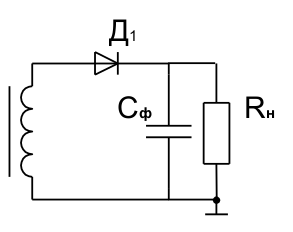
\includegraphics[scale=0.75]{img/diod.png}
		\caption{Однополупериодный \\выпрямитель}\label{figure:2.1:a}
	\end{subfigure}
	\begin{subfigure}[b]{0.35\textwidth}
		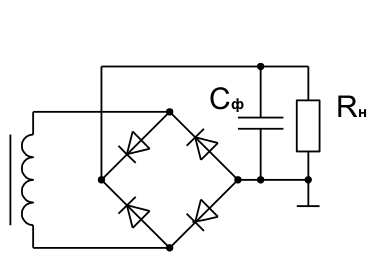
\includegraphics[scale=0.40]{img/4diods.png}
		\caption{Двухполупериодный \\мостовой выпрямитель}\label{figure:2.1:b}
	\end{subfigure}
	\caption{}
\end{figure}

\begin{figure}[H]
	\begin{center}
	\vspace{-0.5cm}
		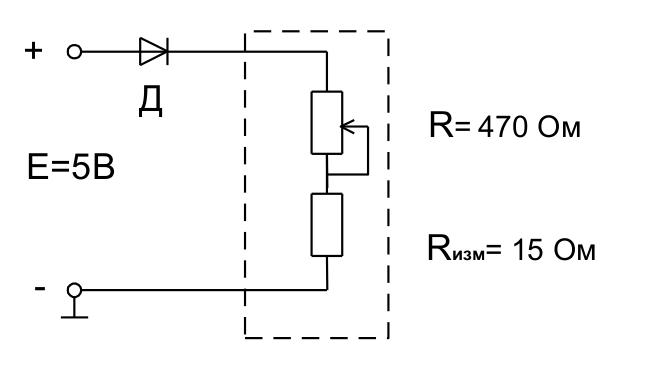
\includegraphics[width=6cm]{img/vah}
		\caption{Цепь для снятия вольт-амперной характеристики}
		\label{figure:2.2} % название для ссылок внутри кода
	\vspace{-0.5cm}
	\end{center}
\end{figure}

\section{Исходные данные}

\begin{table}[H]
	\begin{center}
	\caption{Исходные данные}
	\def\arraystretch{1.4}
		\begin{tabularx}{\textwidth}{|X|X|X|X|X|X|}
			\hline
			$I_\text{н ном}$, мА & $R_\text{изм}$, Ом & $R_\text{н}$, Ом & $C_\text{ф}$, мкФ & Диод\\ \hline
		    120 & 15 & 470 & 1500 & 2Д212А\\\hline	
		\end{tabularx}
		\label{tabular:11}
	\end{center}
\end{table}

%\section{Теоретические зависимости}


\section{Теоретические расчёты}

\begin{equation}
U_\text{н} = U_2 \cdot \sqrt{2}
\end{equation}


\begin{equation}
U_\text{п max} = \frac{I_\text{н} \cdot \Delta t}{C\text{ф}}
\end{equation}

\subsection{Однополупериодный выпрямитель}

\begin{displaymath}
U_\text{н} = U_2 \cdot \sqrt{2} = 6.3 \cdot 1.4 = 8.91 B
\end{displaymath}

\begin{displaymath}
U_\text{п max} = \frac{I_\text{н} \cdot \Delta t}{C\text{ф}} = \frac{120 \cdot 10^{-3}\cdot 20 \cdot 10^{-3}}{1500 \cdot 10^{-6}} = 1.6 B
\end{displaymath}

\subsection{Двухполупериодный выпрямитель}

\begin{displaymath}
U_\text{н} = U_2 \cdot \sqrt{2} = 6.3 \cdot 1.4 = 8.91 B
\end{displaymath}

\begin{displaymath}
U_\text{п max} = \frac{I_\text{н} \cdot \Delta t}{C\text{ф}} = \frac{120 \cdot 10^{-3}\cdot 10 \cdot 10^{-3}}{1500 \cdot 10^{-6}} = 0.8 B
\end{displaymath}

\subsection{Аппроксимация}

Для полученной экспериментальным путем ВАХ диода была выполнена аппроксимация с использованием уравнения Шокли:
\begin{equation}
I = I_0 (e^{\frac{U}{m \phi_t}} - 1).
\end{equation}
Для точек 
$\{\Delta U=0.53\ \text{В}, I_\text{д}=29.3\ \text{мА}\}$ 
и 
$\{\Delta U=0.73\ \text{В}, I_\text{д}=269.3\ \text{мА}\}$ 
из набора экспериментальных данных была получена система уравнений, решением которой являются значения 
$I_0 = 7.99710 \cdot 10^{-5}$ А, $m =  3.47400$.


\section{Экспериментально снятые зависимости}

\subsection{Полупроводниковый диод}

\begin{table}[H]
	\begin{center}
	\caption{ВАХ полупроводникового диода}
	\def\arraystretch{1.2}
		\begin{tabular}{|c|c|c|c|c|}
		\hline 
		\ \ $U_1$, В\ \  & \ \ $U_2$, В\ \  & $\Delta U = U_1 - U_2$, В & \ \ $U_\text{изм}$, В\ \  & \ \ \ $I_\text{д}$, мА\ \ \ \\ 
		\hline 
		5.23 & 4.75 & 0.48 & 0.14 & 9.3 \\ 
		\hline 
		5.21 & 4.68 & 0.53 & 0.44 & 29.3 \\ 
		\hline 
		5.20 & 4.63 & 0.57 & 0.73 & 49.3 \\ 
		\hline 
		5.19 & 4.59 & 0.60 & 1.04 & 69.3 \\ 
		\hline 
		5.18 & 4.56 & 0.62 & 1.35 & 89.3 \\ 
		\hline 
		5.17 & 4.53 & 0.70 & 1.61 & 109.3 \\ 
		\hline 
		5.16 & 4.51 & 0.65 & 1.97 & 129.3 \\ 
		\hline 
		5.15 & 4.49 & 0.66 & 2.24 & 149.3 \\ 
		\hline 
		5.14 & 4.46 & 0.68 & 2.58 & 169.3 \\ 
		\hline 
		5.14 & 4.44 & 0.70 & 2.81 & 189.3 \\ 
		\hline 
		5.12 & 4.41 & 0.68 & 2.98 & 209.3 \\ 
		\hline 
		5.11 & 4.40 & 0.71 & 3.19 & 229.3 \\ 
		\hline 
		5.10 & 4.38 & 0.72 & 3.52 & 249.3 \\ 
		\hline 
		5.10 & 4.37 & 0.73 & 3.91 & 269.3 \\ 
		\hline 
		5.09 & 4.33 & 0.76 & 4.64 & 289.3 \\ 
		\hline 
		\end{tabular} 
		\label{tab:5:1}
	\end{center}
\end{table}

\begin{figure}[H]
	\begin{center}
		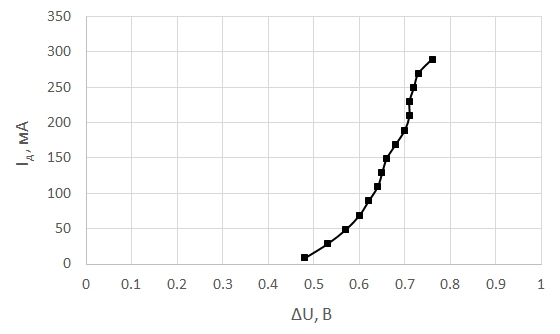
\includegraphics[height=7.5cm]{img/1}
		\caption{Эксперементальная ВАХ полупроводникового диода}
		\label{g:1} % название для ссылок внутри кода
	\end{center}
\end{figure}

\subsection{Однополупериодный выпрямитель}

\begin{table}[H]
	\begin{center}
	\caption{ВАХ однополупериодного выпрямителя}
	\def\arraystretch{1.25}
		\begin{tabular}{|c|c|c|c|}
		\hline 
		\ \ $U_\text{изм}$, В\ \  & \ \ $I_\text{н}$, мА\ \  & \ \ $U_\text{п}$, В\ \  & \ \ $U_\text{н}$, В\ \  \\ \hline
		0.249 & 16 & 9.280 & 0.200 \\ \hline
		0.601 & 41 & 9.080 & 0.432 \\ \hline
		0.899 & 59 & 9.010 & 0.608 \\ \hline
		1.203 & 80 & 8.840 & 0.768 \\ \hline
		1.510 & 100 & 8.790 & 0.984 \\ \hline
		1.832 & 122 & 8.500 & 1.130 \\ \hline
		2.15 & 143 & 8.400 & 1.290 \\ \hline
		2.41 & 160 & 8.240 & 1.490 \\ \hline
		2.70 & 180 & 8.150 & 1.620 \\ \hline
		3.03 & 202 & 8.090 & 1.800 \\ \hline
		3.25 & 217 & 7.990 & 1.920 \\ \hline
		3.68 & 245 & 7.810 & 2.120 \\ \hline
		4.00 & 266 & 7.700 & 2.280 \\ \hline
		4.35 & 290 & 7.490 & 2.480 \\ \hline
		\end{tabular} 
		\label{tab:5:2}
	\end{center}
\end{table}

\begin{figure}[H]
	\begin{center}
		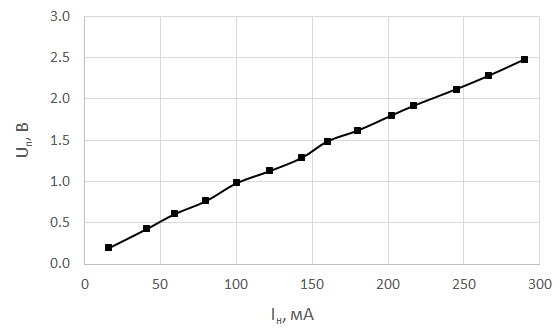
\includegraphics[height=7.5cm]{img/2}
		\caption{Зависимость пульсации напряжения от силы тока нагрузки для однополупериодного выпрямителя}
		\label{g:2} % название для ссылок внутри кода
	\end{center}
\end{figure}

\begin{figure}[H]
	\begin{center}
		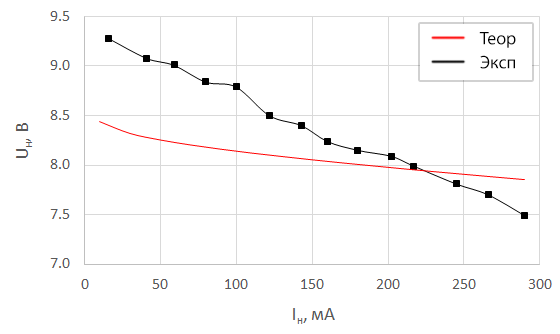
\includegraphics[height=7.5cm]{img/3}
		\caption{Зависимость напряжения нагрузки от силы тока нагрузки для однополупериодного выпрямителя}
		\label{g:3} % название для ссылок внутри кода
	\end{center}
\end{figure}



Вычислим $U_\text{н}$ при $I_\text{н}$ = 120 мА. Для этого построим интерполяционный полином и посчитаем его значение в точке 120.

$U_\text{н}$ = 8.504 В

Вычислим $U_\text{п max}$ при $I_\text{н}$ = 120 мА. Для этого построим интерполяционный полином и посчитаем его значение в точке 120.

$U_\text{п max}$ = 1.116 В

\subsection{Двухполупериодный выпрямитель}

\begin{table}[H]
	\begin{center}
	\caption{ВАХ двухполупериодного диода}
	\def\arraystretch{1.0}
		\begin{tabular}{|c|c|c|c|}
		\hline 
		\ \ $U_\text{изм}$, В\ \  & \ \ $I_\text{н}$, мА\ \  & \ \ $U_\text{п}$, В\ \  & \ \ $U_\text{н}$, В\ \  \\ \hline
		0.251 & 16 & 0.140 & 8.95 \\ \hline
		0.602 & 39 & 0.236 & 8.92 \\ \hline
		0.893 & 60 & 0.323 & 8.83 \\ \hline
		1.205 & 79 & 0.433 & 8.78 \\ \hline
		1.511 & 104 & 0.520 & 8.57 \\ \hline
		1.874 & 125 & 0.591 & 8.47 \\ \hline
		2.23 & 149 & 0.679 & 8.25 \\ \hline
		2.61 & 174 & 0.780 & 8.23 \\ \hline
		2.92 & 209 & 0.884 & 8.09 \\ \hline
		3.46 & 242 & 1.05 & 7.96 \\ \hline
		4.08 & 273 & 1.15 & 7.79 \\ \hline
		4.49 & 291 & 1.20 & 7.63 \\ \hline
		\end{tabular} 
		\label{tab:5:3}
	\end{center}
\end{table}

\begin{figure}[H]
	\begin{center}
		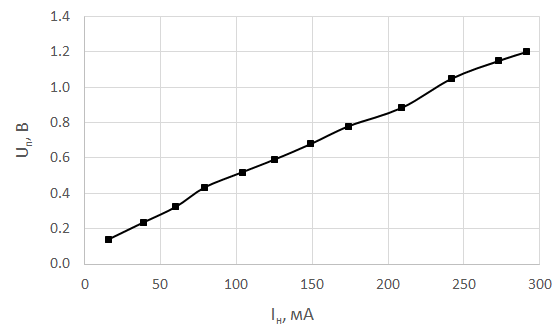
\includegraphics[height=7.5cm]{img/4}
		\caption{Зависимость пульсации напряжения от силы тока нагрузки для двухполупериодного выпрямителя}
		\label{g:4} % название для ссылок внутри кода
	\end{center}
\end{figure}

\begin{figure}[H]
	\begin{center}
		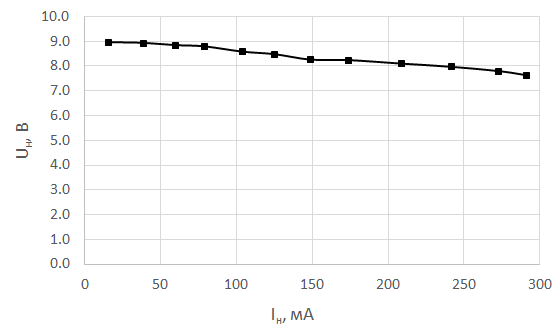
\includegraphics[height=7.5cm]{img/5}
		\caption{Зависимость напряжения нагрузки от силы тока нагрузки для двухполупериодного выпрямителя}
		\label{g:5} % название для ссылок внутри кода
	\end{center}
\end{figure}

Вычислим $U_\text{н}$ при $I_\text{н}$ = 120 мА. Для этого построим интерполяционный полином и посчитаем его значение в точке 120.

$U_\text{н}$ = 8.501 В

Вычислим $U_\text{п max}$ при $I_\text{н}$ = 120 мА. Для этого построим интерполяционный полином и посчитаем его значение в точке 120.

$U_\text{п max}$ = 0.574 В

\section{Погрешности}

\subsection{Предельно допустимые}

Номинальное значение емкости конденсатора может отклоняться от реального на 20\% в меньшую сторону и на 80\% в большую. С учетом того, что пульсация напряжения обратно пропорциональна емкости конденсатора, предельно допустимая погрешность $\delta U_\text{п}$ равна 80\% при отклонении в меньшую сторону и 20\% при отклонении в большую.

\subsection{Однополупериодный выпрямитель}

$\delta U_\text{п max} = \frac{U_\text{п max\ \ теор} - U_\text{п max\ \ эксп}}{U_\text{п max\ \ теор}} = \frac{1.6 - 1.116}{1.6} = 0.302 = 30.2 \%$

$\delta U_\text{н} = \frac{U_\text{н\ \ теор} - U_\text{н\ \ эксп}}{U_\text{н\ \ теор}} = \frac{8.91 - 8.504}{8.91} = 0.045 = 4.5 \%$

\subsection{Двухполупериодный выпрямитель}

$\delta U_\text{п max} = \frac{U_\text{п max\ \ теор} - U_\text{п max\ \ эксп}}{U_\text{п max\ \ теор}} = \frac{0.8 - 0.574}{0.8} = 0.282 = 28.2 \%$

$\delta U_\text{н} = \frac{U_\text{н\ \ теор} - U_\text{н\ \ эксп}}{U_\text{н\ \ теор}} = \frac{8.91 - 8.501}{8.91} = 0.046 = 4.6 \%$

\section{Выводы}

 Приведенные погрешности $U_\text{п}$ для однополупериодного и двухполупериодного выпрямителей равны 30.2\% и 28.2\% соответственно, что не превышает предельно допустимую погрешность - 80\%.

Таким образом, теоретические формулы 4.1 и 4.2 являются верными.

\end{document}
